\documentclass[11pt,a4paper]{article}
\usepackage{amsmath}
\usepackage{amssymb}
\usepackage{graphicx}
\usepackage{subfigure}
\usepackage{float}
\usepackage{xeCJK}
\usepackage{geometry}
\geometry{left=2.0cm,right=2.0cm,top=2.0cm,bottom=2.0cm}

\title{Energy transfer in ITG/KBM system}
\author{Guangzhi Ren}
\date{\today}

\begin{document}

\maketitle

\section{model equation}

\begin{equation}
 	\frac{dn}{dt}=a\frac{dn_{eq}}{dr}-n_{eq}\nabla_{\parallel}v+\nabla_{\parallel}j+\omega_d(n_{eq}\phi-p_e)+D_n\nabla^2_\perp{n}
\end{equation}

\begin{equation}
	\frac{d\nabla^2_\perp\phi}{dt}=-aT_{eq}(\frac{1}{n}\frac{dn_{eq}}{dr}+\frac{1}{T_{eq}}\frac{dT_{eq}}{dr})\nabla_\theta\nabla^2_\perp\phi+\frac{1}{n_{eq}}\nabla_{\parallel}j-\omega_d(T_i+\frac{T_{eq}}{n_{eq}}n+\frac{p_e}{n_{eq}})+D_U\nabla^4_\perp\phi
\end{equation}

\begin{equation}
\frac{dv}{dt}=-\nabla_\parallel{T_i}-2\frac{T_{eq}}{n_{eq}}\nabla_\parallel{n}-\beta{aT_{eq}}(\frac{2}{n_{eq}}\frac{dn_{eq}}{dr}+\frac{1}{T_{eq}}\frac{dT_{eq}}{dr})\nabla_\theta{A}+D_v\nabla^2_\perp{v}
\end{equation}

\begin{equation}
\beta\frac{\partial{A}}{\partial{t}}=-\nabla_\parallel\phi+\frac{T_{eq}}{n_{eq}}\nabla_\parallel{n}+\beta{aT_{eq}}\frac{1}{n_{eq}}\frac{dn_{eq}}{dr}\nabla_\theta{A}+\sqrt{\frac{\pi}{2}\frac{m_e}{m_i}}|\nabla_{\parallel}|(v-\frac{j}{n_{eq}})-\eta{j}
\end{equation}

\begin{equation}
\frac{dT_i}{dt}=...
\end{equation}


\section{energy balance equation}


\section{zonal flow character}
	\begin{figure}[H]
		\centering
		\subfigure[]{
			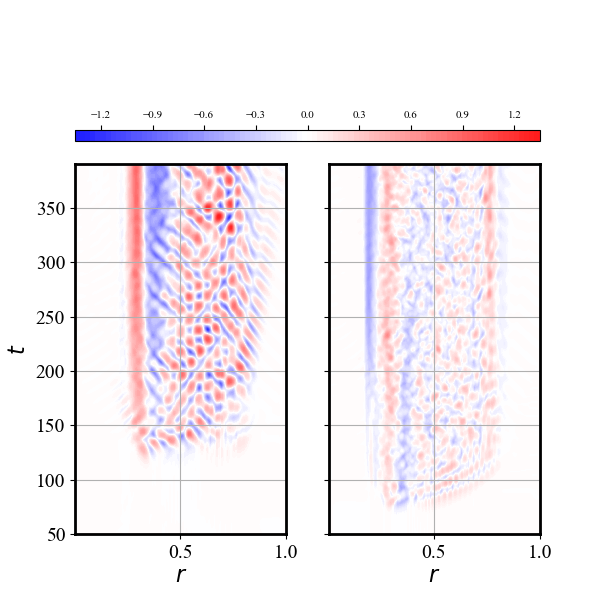
\includegraphics[width=0.35\textwidth]{./images/zf_contour.png} 
		}
		\subfigure[]{
			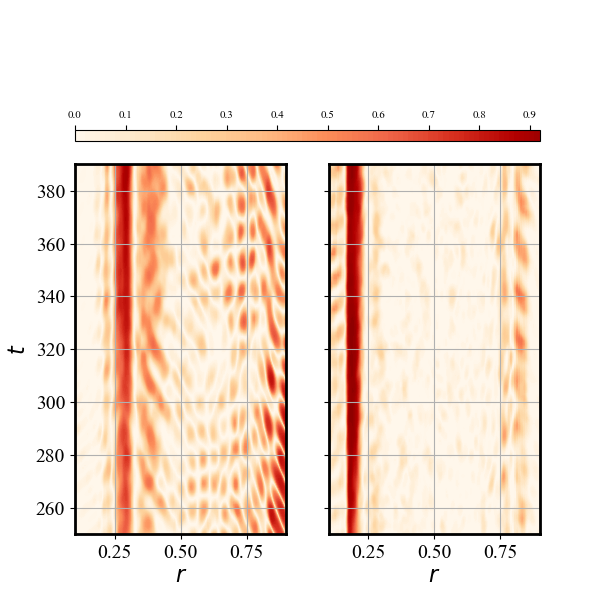
\includegraphics[width=0.35\textwidth]{./images/zf_ratio.png}
		}
		\caption{(a)zonal flow as a function of radius and time,(b)$E_{k,ZF}/E_{k,all}$as a function of radius and time}
	\end{figure}

\section{energy drive of $E_{k,m=0,n=0}$ and $E_{p,m=1,n=0}$}




\end{document}
